\documentclass[12pt]{article}

\usepackage[a4paper,top=1in,bottom=1in,left=1in,right=1in]{geometry}

\usepackage[utf8]{inputenc}
\usepackage{float}
\usepackage{amsmath}
\usepackage{graphicx}
\usepackage{titlesec}
\usepackage{tcolorbox}
\usepackage{enumitem}
\usepackage{tikz}
\usetikzlibrary{patterns}
\usetikzlibrary{graphs}
\usetikzlibrary{graphdrawing}
\usegdlibrary{force}
\usepackage{amssymb}
\usepackage{hyperref}

\title{\bfseries Laborator Proiectare Logică 6}
\author{Sîrghe Matei}
\date{November 20, 2024}

\titleformat{\section}
  {\normalfont\Large\bfseries}{\thesection}{1em}{}
\begin{document}
\maketitle

\begin{center}
    \large{\textbf{Half Adder}}
\end{center}

\renewcommand{\arraystretch}{1}

\begin{figure}[h!]
    \begin{minipage}{0.8\textwidth}
       $S=\sum(1,2)=\bar{A}B+A\bar{B}$\\
       $S=\Pi(0,3)=(A+B)(\bar{A}+\bar{B})$\\
       $S=A\bigoplus B$\\
       $C_{o}=\sum(3)=AB$\\
       $C_{o}=\Pi(0,1,2)=(A+B)(A+\bar{B})(\bar{A}+B)$\\
    \end{minipage}
    \hfill
    \begin{minipage}{0.18\textwidth}
        \begin{tabular}{|c|c|c|c|}
            \hline
            A & B & S & $C_{o}$ \\ \hline
            0 & 0 & 0 & 0 \\ \hline
            0 & 1 & 1 & 0 \\ \hline
            1 & 0 & 1 & 0 \\ \hline
            1 & 1 & 0 & 1 \\ \hline
        \end{tabular}
    \end{minipage}
\end{figure}

\begin{figure}[h!]
    \begin{minipage}{0.5\textwidth}
        \begin{tikzpicture}
            \draw (0,0) grid (2,-2);
            \draw[-] (0,0) -- (-0.5,0.5);
            \node at (-0.5, 0.2) {S};

            \node at (0.5, -0.5) {0};
            \node at (1.5, -0.5) {1};
            %
            \node at (0.5, -1.5) {1};
            \node at (1.5, -1.5) {0};

            \node at (0.5, 0.5) {0};
            \node at (1.5, 0.5) {1};
            \node at (-0.5, -0.5) {0};
            \node at (-0.5, -1.5) {1};

        \end{tikzpicture}
    \end{minipage}
    \hfill
    \begin{minipage}{0.5\textwidth}
        \begin{tikzpicture}
            \draw (0,0) grid (2,-2);
            \draw[-] (0,0) -- (-0.5,0.5);
            \node at (-0.5, 0.2) {$C_{o}$};

            \node at (0.5, -0.5) {0};
            \node at (1.5, -0.5) {0};
            %
            \node at (0.5, -1.5) {0};
            \node at (1.5, -1.5) {1};

            \node at (-0.5, -0.5) {0};
            \node at (-0.5, -1.5) {1};
            \node at (0.5, 0.5) {0};
            \node at (1.5, 0.5) {1};

        \end{tikzpicture}
    \end{minipage}
\end{figure}

\begin{figure}[h!]
    \begin{minipage}{0.4\textwidth}
        \begin{tikzpicture}
            \draw[-] (0,0) -- (3,0);
            \draw[-] (3,0) -- (3,-3);
            \draw[-] (3,-3) -- (0,-3);
            \draw[-] (0,-3) -- (0,0);

            \node at (0.5, -0.5) {A};
            \node at (2.5, -0.5) {S};
            \node at (2.5, -2.5) {$C_{o}$};
            \node at (0.5, -2.5) {B};
            \node at (1.5, -1.5) {$H_{A}$};

        \end{tikzpicture}
    \end{minipage}
    \hfill
    \begin{minipage}{0.5\textwidth}
        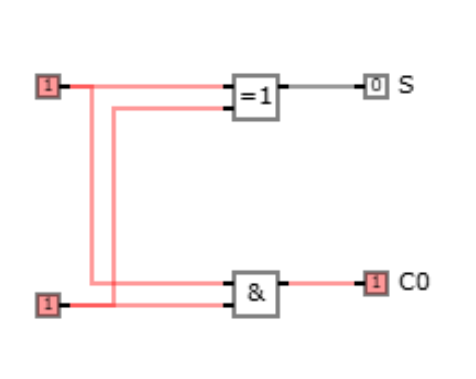
\includegraphics[scale=0.6]{Schema1.png}
    \end{minipage}
\end{figure}

\newpage
\begin{center}
    \large{\textbf{Full Adder}}
\end{center}

\begin{figure}[h!]
    \begin{minipage}{0.7\textwidth}
       $S=\sum(1,2,4,7)=\bar{A}\bar{B}C_{i}+\bar{A}B\bar{C_{i}}+\bar{A}\bar{B}\bar{C_{i}}+A\bar{B}\bar{C_{i}}+ABC_{i}$\\
       $S=\Pi(0,3,5,6)$\\
       $=(A+\bar{B}+C_{i})(A+\bar{B}+C_{i})(\bar{A}+B+\bar{C_{i}})(\bar{A}+\bar{B}+C_{i})$\\
       $S=\bar{C_{i}}(\bar{A}B+A\bar{B})+C_{i}(\bar{A}\bar{B}+AB)$\\
       $A\bigoplus B=\bar{A}B+A\bar{B}$\\
       $A\bigoplus B=\bar{A}\bar{B}+AB$\\
       $S=A\bigoplus B\bigoplus C$\\
    \end{minipage}
    \hfill
    \begin{minipage}{0.28\textwidth}
        \begin{tabular}{|c|c|c|c|c|}
            \hline
            A & B & $C_{i}$ & S & $C_{o}$ \\ \hline
            0 & 0 & 0 & 0 & 0 \\ \hline
            0 & 0 & 1 & 1 & 0 \\ \hline
            0 & 1 & 0 & 1 & 0 \\ \hline
            0 & 1 & 1 & 0 & 1 \\ \hline
            1 & 0 & 0 & 1 & 0 \\ \hline
            1 & 0 & 1 & 0 & 1 \\ \hline
            1 & 1 & 0 & 0 & 1 \\ \hline
            1 & 1 & 1 & 1 & 1 \\ \hline
        \end{tabular}
    \end{minipage}
\end{figure}

\begin{figure}[h!]
    \begin{minipage}{0.5\textwidth}
        \begin{tikzpicture}
            \draw (0,0) grid (4,-2);
            \draw[-] (0,0) -- (-1,1);
            \node at (-0.75, 0.25) {$C_{i}$};
            \node at (-0.25, 0.75) {$AB$};
            \node at (-1.25, 1.25) {$S$};

            \draw[thick] (0.5, -1.5) ellipse (0.5cm and 0.5cm);
            \draw[thick] (2.5, -1.5) ellipse (0.5cm and 0.5cm);
            \draw[thick] (1.5, -0.5) ellipse (0.5cm and 0.5cm);
            \draw[thick] (3.5, -0.5) ellipse (0.5cm and 0.5cm);
        
            \node at (0.5, -0.5) {0};
            \node at (1.5, -0.5) {1};
            \node at (2.5, -0.5) {0};
            \node at (3.5, -0.5) {1};
            %
            \node at (0.5, -1.5) {1};
            \node at (1.5, -1.5) {0};
            \node at (2.5, -1.5) {1};
            \node at (3.5, -1.5) {0};
        
            \node at (-0.5, -0.5) {0};
            \node at (-0.5, -1.5) {1};
            \node at (0.5, 0.5) {00};
            \node at (1.5, 0.5) {01};
            \node at (2.5, 0.5) {11};
            \node at (3.5, 0.5) {10};
        \end{tikzpicture}
    \end{minipage}
    \hfill
    \begin{minipage}{0.5\textwidth}
        \begin{tikzpicture}
            \draw (0,0) grid (4,-2);
            \draw[-] (0,0) -- (-1,1);
            \node at (-0.75, 0.25) {$C_{i}$};
            \node at (-0.25, 0.75) {$AB$};
            \node at (-1.25, 1.25) {$C_{o}$};

            \draw[thick] (2, -1.5) ellipse (1cm and 0.5cm);
            \draw[thick] (3, -1.5) ellipse (1cm and 0.5cm);
            \draw[thick] (2.5, -1) ellipse (0.5cm and 1cm);
        
            \node at (0.5, -0.5) {0};
            \node at (1.5, -0.5) {0};
            \node at (2.5, -0.5) {1};
            \node at (3.5, -0.5) {0};
            %
            \node at (0.5, -1.5) {0};
            \node at (1.5, -1.5) {1};
            \node at (2.5, -1.5) {1};
            \node at (3.5, -1.5) {1};
        
            \node at (-0.5, -0.5) {0};
            \node at (-0.5, -1.5) {1};
            \node at (0.5, 0.5) {00};
            \node at (1.5, 0.5) {01};
            \node at (2.5, 0.5) {11};
            \node at (3.5, 0.5) {10};
        \end{tikzpicture}
    \end{minipage}
\end{figure}

\begin{figure}[h!]
    \begin{minipage}{0.6\textwidth}
        $C_{o}=\sum(3,5,6,7)=\bar{A}BC_{i}+A\bar{B}C_{i}+AB\bar{C_{i}}+ABC_{i}$\\
       $C_{o}=\Pi(0,1,2,4)=(A+B+C_i)(A+B+\bar{C_i})(A+\bar{B}+C_i)(\bar{A}+B+C_i)$\\
       $C_{o}=AB+BC_i+AC_i$\\
       $C_{o}=AB+C_{i}(A+B)$\\
    \end{minipage}
    \hfill
    \begin{minipage}{0.3\textwidth}
        \begin{tikzpicture}
            \draw[-] (0,0) -- (3,0);
            \draw[-] (3,0) -- (3,-3);
            \draw[-] (3,-3) -- (0,-3);
            \draw[-] (0,-3) -- (0,0);

            \node at (0.5, -0.5) {A};
            \node at (2.5, -0.5) {S};
            \node at (2.5, -2.5) {$C_{o}$};
            \node at (0.5, -2.5) {$C_{i}$};
            \node at (0.5, -1.5) {B};
            \node at (1.5, -1.5) {$F_{A}$};
        \end{tikzpicture}
    \end{minipage}
\end{figure}

\begin{minipage}{1\textwidth}
    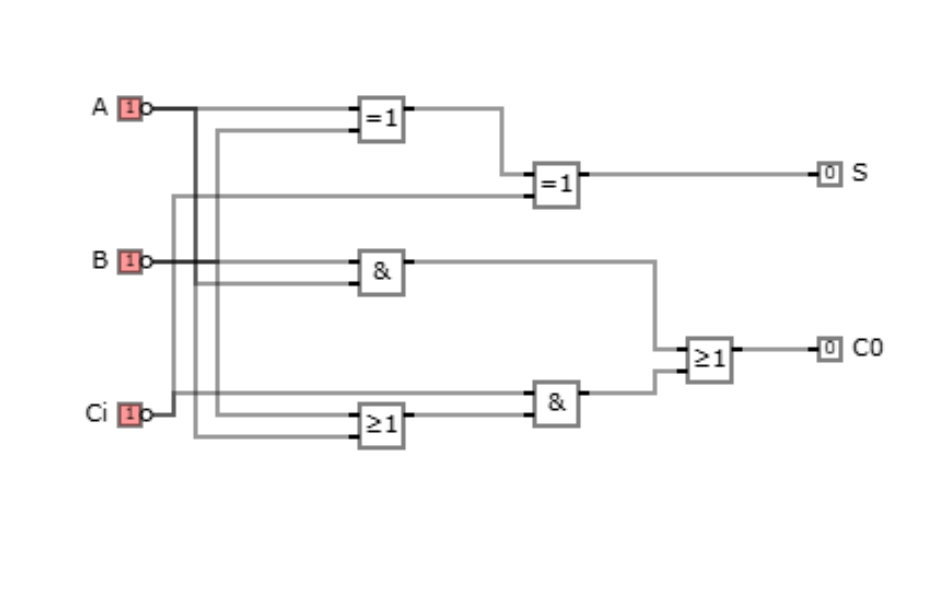
\includegraphics[scale=0.6]{Schema2.png}
\end{minipage}

\newpage
\begin{center}
    \large{\textbf{Half Subtractor}}
\end{center}

\begin{figure}[h!]
    \begin{minipage}{0.7\textwidth}
       $D=\sum(1,2)=\bar{A}B+A\bar{B}=A\bigoplus B$\\
       $D=\Pi(0,3)=(A+B)(\bar{A}+\bar{B})=A\bigoplus B$\\
       $B_{o}=\sum(1)=\bar{A}B$\\
       $B_{o}=\Pi(0,2,3)$\\
       $B_{o}=(A+B)(\bar{A}+B)(\bar{A}+\bar{B})=\bar{A}B$\\
    \end{minipage}
    \hfill
    \begin{minipage}{0.28\textwidth}
        \begin{tabular}{|c|c|c|c|}
            \hline
            A & B & D & $B_{o}$ \\ \hline
            0 & 0 & 0 & 0 \\ \hline
            0 & 1 & 1 & 1 \\ \hline
            1 & 0 & 1 & 0 \\ \hline
            1 & 1 & 0 & 0 \\ \hline
        \end{tabular}
    \end{minipage}
\end{figure}

\begin{figure}[h!]
    \begin{minipage}{0.7\textwidth}
        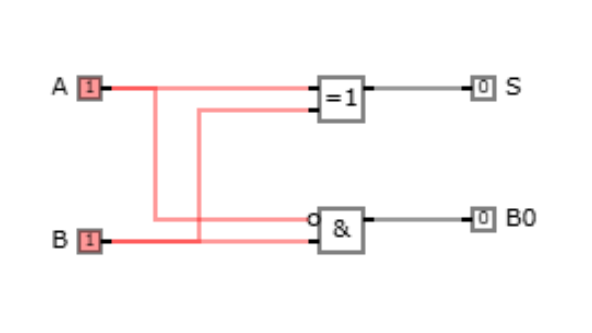
\includegraphics[scale=0.6]{Schema3.png}
    \end{minipage}
    \hfill
    \begin{minipage}{0.28\textwidth}
        \begin{tikzpicture}
            \draw[-] (0,0) -- (3,0);
            \draw[-] (3,0) -- (3,-3);
            \draw[-] (3,-3) -- (0,-3);
            \draw[-] (0,-3) -- (0,0);

            \node at (0.5, -0.5) {A};
            \node at (2.5, -0.5) {D};
            \node at (2.5, -2.5) {$B_{o}$};
            \node at (0.5, -2.5) {B};
            \node at (1.5, -1.5) {$H_{S}$};
        \end{tikzpicture}
    \end{minipage}
\end{figure}

\newpage
\begin{center}
    \large{\textbf{Full Subtractor}}
\end{center}

\begin{figure}[h!]
    \begin{minipage}{0.7\textwidth}
       $D=\sum(1,2,4,7)=A\bigoplus B\bigoplus B_i$\\
       $D=\Pi(0,3,5,6)=A\bigoplus B\bigoplus B_i$\\
       $B_o=\sum(1,2,3,7)$\\
       $B_o=\bar{A}\bar{B}B_i+\bar{A}B\bar{B_i}+\bar{A}BB_{i}+ABB_{i}$\\
       $B_o=\Pi(0,4,5,6)$\\
       $B_o=(A+B+B_i)(\bar{A}+B+B_i)(\bar{A}+B+\bar{B_i})(\bar{A}+\bar{B}+B_i)$\\
    \end{minipage}
    \hfill
    \begin{minipage}{0.28\textwidth}
        \begin{tabular}{|c|c|c|c|c|}
            \hline
            A & B & $B_{i}$ & D & $B_{o}$ \\ \hline
            0 & 0 & 0 & 0 & 0 \\ \hline
            0 & 0 & 1 & 1 & 1 \\ \hline
            0 & 1 & 0 & 1 & 1 \\ \hline
            0 & 1 & 1 & 0 & 1 \\ \hline
            1 & 0 & 0 & 1 & 0 \\ \hline
            1 & 0 & 1 & 0 & 0 \\ \hline
            1 & 1 & 0 & 0 & 0 \\ \hline
            1 & 1 & 1 & 1 & 1 \\ \hline
        \end{tabular}
    \end{minipage}
\end{figure}

\begin{figure}[h!]
    \begin{minipage}{0.6\textwidth}
        \begin{tikzpicture}
            \draw (0,0) grid (4,-2);
            \draw[-] (0,0) -- (-1,1);
            \node at (-0.75, 0.25) {$B_{i}$};
            \node at (-0.25, 0.75) {$AB$};
            \node at (-1.25, 1.25) {$B_{o}$};
        
            \draw[thick] (1.5, -1) ellipse (0.5cm and 1cm);
            \draw[thick] (1, -1.5) ellipse (1cm and 0.5cm);
            \draw[thick] (2, -1.5) ellipse (1cm and 0.5cm);
        
            \node at (0.5, -0.5) {0};
            \node at (1.5, -0.5) {1};
            \node at (2.5, -0.5) {0};
            \node at (3.5, -0.5) {0};
            %
            \node at (0.5, -1.5) {1};
            \node at (1.5, -1.5) {1};
            \node at (2.5, -1.5) {1};
            \node at (3.5, -1.5) {0};
        
            \node at (-0.5, -0.5) {0};
            \node at (-0.5, -1.5) {1};
            \node at (0.5, 0.5) {00};
            \node at (1.5, 0.5) {01};
            \node at (2.5, 0.5) {11};
            \node at (3.5, 0.5) {10};
        \end{tikzpicture}
    \end{minipage}
    \hfill
    \begin{minipage}{0.4\textwidth}
        $B_{o}=\bar{A}B+\bar{A}B_i+BB_i$\\
        $B_{o}=\bar{A}B+B_i(\bar{A}+B)$\\
    \end{minipage}
\end{figure}

\begin{figure}[h!]
    \begin{minipage}{0.7\textwidth}
        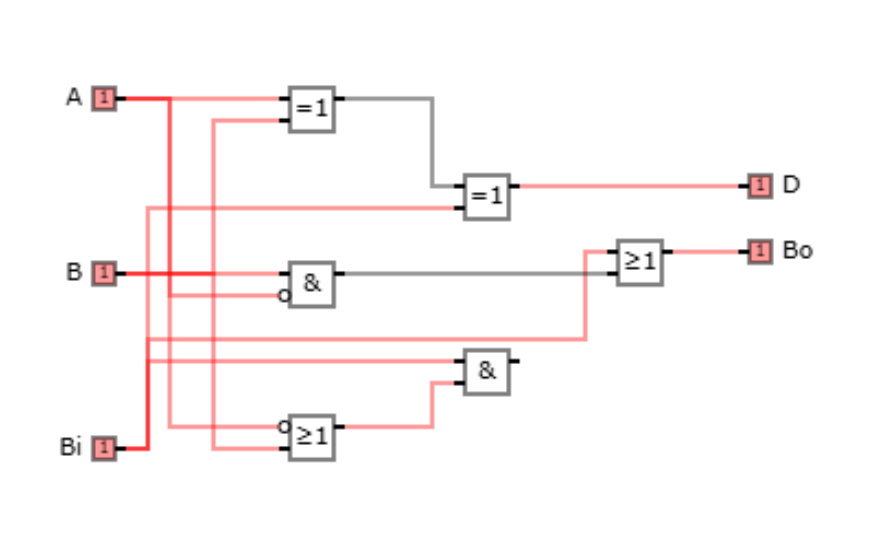
\includegraphics[scale=0.5]{Schema4.png}
    \end{minipage}
    \hfill
    \begin{minipage}{0.28\textwidth}
        \begin{tikzpicture}
            \draw[-] (0,0) -- (3,0);
            \draw[-] (3,0) -- (3,-3);
            \draw[-] (3,-3) -- (0,-3);
            \draw[-] (0,-3) -- (0,0);

            \node at (0.5, -0.5) {A};
            \node at (2.5, -0.5) {D};
            \node at (2.5, -2.5) {$B_{o}$};
            \node at (0.5, -2.5) {$B_{i}$};
            \node at (0.5, -1.5) {B};
            \node at (1.5, -1.5) {$F_{D}$};
        \end{tikzpicture}
    \end{minipage}
\end{figure}

\end{document}